\documentclass[10pt]{article}
\usepackage{fullpage,enumitem,amsmath,amssymb,graphicx,listings,tikz,bbm,xcolor}
\setlength{\parindent}{0pt}

\begin{document}

\begin{center}
{\Large \textbf{Theory Problems: Batch 2}}

\begin{tabular}{rl}
\\
Course: & Coursera Algorithms Specialization \\
Name: & Bryan Yaggi
\end{tabular}
\end{center}

\section*{\normalsize Problem 1}

Prove that the worst-case expected running time of every randomized comparison-based sorting algorithm is $\Omega(n \log ⁡n)$. (Here the worst-case is over inputs, and the expectation is over the random coin flips made by the algorithm.)
\bigskip

In lecture, we showed that any deterministic comparison-based sorting algorithm has a lower bound, $\Omega(n log n)$. First, prove the average-case time is $\Omega(n log n)$. A comparison-based sorting algorithm can be represented as a binary decision tree. See the following example.
\smallskip

Example: Given three elements in a list, $[e_1, e_2, e_3]$.

\begin{center}
  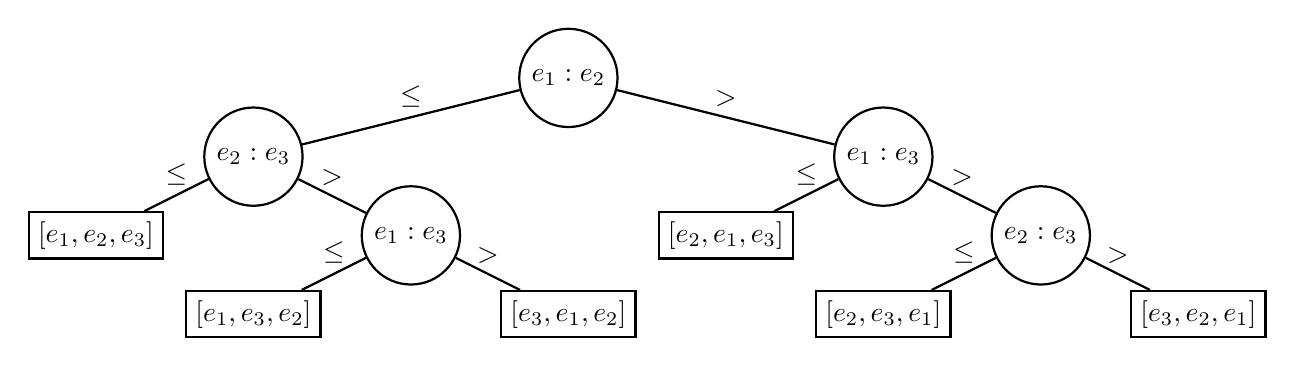
\begin{tikzpicture}
		\begin{scope}[every node/.style={circle,thick,draw}]
    		\node (C11) at (0,0) {$e_1:e_2$};
    		\node (C21) at (-4,-1) {$e_2:e_3$};
    		\node (C22) at (4,-1) {$e_1:e_3$};
    		\node (C31) at (-2,-2) {$e_1:e_3$};
    		\node (C32) at (6,-2) {$e_2:e_3$};
		\end{scope}
		\begin{scope}[every node/.style={thick,draw}]
    		\node (L1) at (-6,-2) {$[e_1, e_2, e_3]$};
    		\node (L3) at (-4,-3) {$[e_1, e_3, e_2]$};
    		\node (L4) at (0,-3) {$[e_3, e_1, e_2]$};
    		\node (L2) at (2,-2) {$[e_2, e_1, e_3]$};
    		\node (L5) at (4,-3) {$[e_2, e_3, e_1]$};
    		\node (L6) at (8,-3) {$[e_3, e_2, e_1]$};
		\end{scope}
		\begin{scope}[every edge/.style={draw=black,thick}]
			\path [-] (C11) edge node [above] {$\leq$} (C21);
			\path [-] (C11) edge node [above] {$>$} (C22);
			\path [-] (C21) edge node [above] {$>$} (C31);
			\path [-] (C22) edge node [above] {$>$} (C32);
			\path [-] (C21) edge node [above] {$\leq$} (L1);
			\path [-] (C22) edge node [above] {$\leq$} (L2);
			\path [-] (C31) edge node [above] {$\leq$} (L3);
			\path [-] (C31) edge node [above] {$>$} (L4);
			\path [-] (C32) edge node [above] {$\leq$} (L5);
			\path [-] (C32) edge node [above] {$>$} (L6);
		\end{scope}
	\end{tikzpicture}
\end{center}

For $n$ elements, there are $n!$ possible permutations, and each permutation has a $\frac{1}{n!}$ probability of being reached. Let $D(T)$ be the external path length of the decision tree, $T$, or the sum of the depths of each leaf in the tree. For any $T$ with $k > 1$ leaves, $D(T) = D(LT) + D(RT) + k$, where $LT$ and $RT$ are the left and right subtrees, respectively. This is true because the leaves of $LT$ and $RT$ are one node shallower than in $T$, and the path to each leaf must go through the root node. Using this observation, the combination of leaves in $LT$ and $RT$ that minimizes $D(T)$ can be found. $D(T) \geq i \log i + (k - i) \log (k - i) + k$ where $i$ is the number of leaves in $LT$.

\begin{align*}
	D(T) &\geq i \log i + (k - i) \log (k - i) + k \\
	\frac{\partial D(T)}{\partial i} &= \log i + 1 - \log(k - i) - 1 = \log \frac{i}{k - i} \\
	\frac{\partial D(T)}{\partial i} &= 0 \iff \frac{i}{k - i} = 1 \implies i = \frac{k}{2}
\end{align*}

This result indicates that $D(T)$ is minimized by a balanced tree. Therefore, $D(T) > k \log k \iff D(T) > n! \log (n!)$. The average-case time, or leaf depth, for sorting $n$ elements is $\log(n!) \implies \Omega(n \log n)$. Now, show the expected running time for random camparison-based sort. A random comparison sort is just a randomly-selected decision tree, $T$ from the set valid decision trees for sorting the input. Let $N$ be the number of valid decision trees.

\begin{align*}
	E(time) &= \sum_{j = 1}^{N} p_j time = \sum_{j = 1}^{N} \frac{1}{N} \Omega(n \log n) \\
	&= \Omega(n \log n)
\end{align*}

\smallskip

See CLRS Problem 8-1 and solution.

\section*{\normalsize Problem 2}

Suppose we modify the deterministic linear-time selection algorithm by grouping the elements into groups of 7, rather than groups of 5. (Use the ``median-of-medians" as the pivot, as before.) Does the algorithm still run in $O(n)$ time? What if we use groups of 3?
\bigskip

Answer...

\section*{\normalsize Problem 3}

Given an array of $n$ distinct (but unsorted) elements $x_1, x_2, \dots, x_n$​ with positive weights $w_1, w_2, \dots, w_n$​ such that $\sum_{i=1}^{n} w_i = W$, a weighted median is an element $x_k$​ for which the total weight of all elements with value less than $x_k$​ (i.e., $\sum_{x_i < x_k}$) is at most $W/2$, and also the total weight of elements with value larger than $x_k$​ (i.e., $\sum_{x_i > x_k}$) is at most $W/2$. Observe that there are at most two weighted medians. Show how to compute all weighted medians in $O(n)$ worst-case time.
\bigskip

Answer...

\section*{\normalsize Problem 4}

We showed in an optional video lecture that every undirected graph has only polynomially (in the number $n$ of vertices) different minimum cuts. Is this also true for directed graphs? Prove it or give a counterexample.
\bigskip

Answer...

\section*{\normalsize Problem 5}

For a parameter $\alpha \geq 1$, an $\alpha$-minimum cut is one for which the number of crossing edges is at most $\alpha$ times that of a minimum cut. How many $\alpha$-minimum cuts can an undirected graph have, as a function of $\alpha$ and the number $n$ of vertices? Prove the best upper bound that you can.
\bigskip

Answer...

\end{document}
